\chapter{Practical examples}
\label{chapter3}
% \thispagestyle{empty}

remove: \citep{paper:pacs}

\noindent 
\section{Application to particle-size curves in heterogeneous aquifers}
We consider here a data set, kindly provided by professor Menafoglio, obtained at the Lauswiesen site, located in the Neckar river valley, near the city of T\"{u}bingen (Germany). 
The subsurface system in the area has been characterized through extensive information obtained at a number of boreholes, which are employed to perform sedimentological as well as hydraulic analyses.

Of specific relevance to our study are the available 406 particle-size curves (PSCs) sampled along 12 fully penetrating vertical boreholes.

A set of twelve discrete sieve diameters (i.e., 0.063, 0.125, 0.25, 0.50,
1.0, 2.0, 4.0, 8.0, 16.0, 31.5, 63.0 and 100.0 mm) were employed to reconstruct these curves by way of grain sieve analysis on soil samples.

Figure \ref{fig:boreholes} depicts a sketch of the borehole network and sampling locations at the site. 

\begin{figure}
	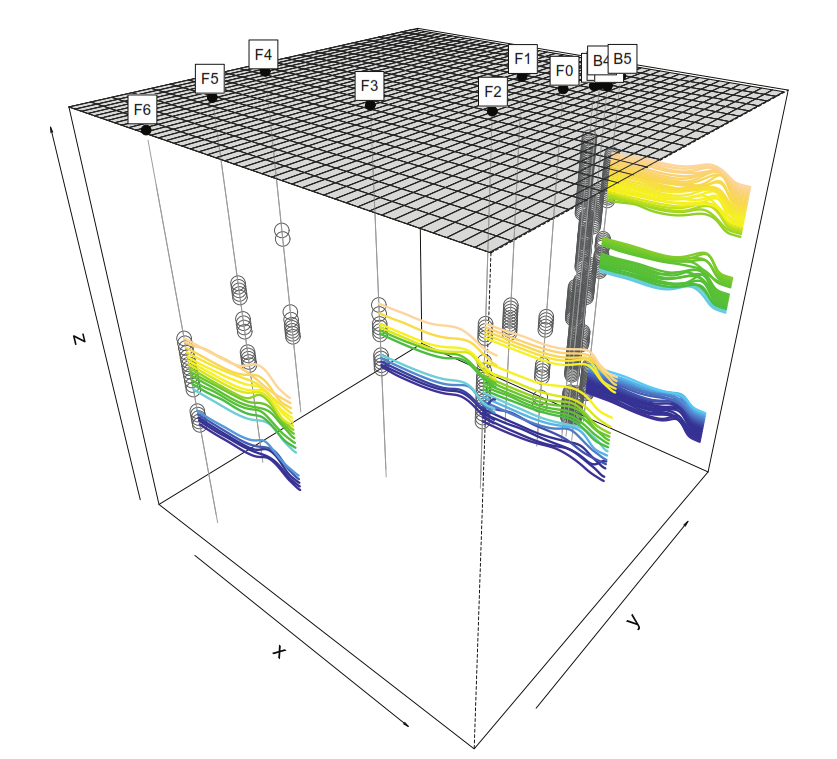
\includegraphics[width=8cm]{./pictures/particle_size_densities.png}
	\centering
	\caption{Three-dimensional representation of particle-size densities at the Lauswiesen site. Grey points represent measurement locations, colored curves represent a subset of the dataset of PSDs. Colors indicate the ordering of the curves along the borehole.}
\label{fig:boreholes}	
\end{figure}

Reconstructed particle-size densities can be employed, as in \citep{menafoglio:psc}, to perform a geostatistical analysis, in order to classify PSCs into clusters which represent the occurrence at a site of diverse soil types, to characterize the spatial distribution of each identified textural class, and to provide Kriging estimates of the heterogeneous distribution of PSCs at unsampled locations.

PSDs describe the local distributions of grain sizes 
within the aquifer system. From the mathematical viewpoint, a 
particle-size density is a probability density function, associated 
with the distribution of particle sizes within a given soil sample. 
As such, available data consist of a set of constrained curves, spatially distributed. The statistical characterization of PSDs plays a key role in the classification of soil types, for inferring hydraulic parameters (e.g., porosity and hydraulic conductivity), and reconstructing the internal architecture of the groundwater system. In this vein, the analysis of PSDs may be concerned with, e.g., (a) the classification of PSDs to identify geomaterials at the site, and (b) 








%---------------------------------------------------------------




